%% ****** Start of file template.aps ****** %
%%
%%
%%   This file is part of the APS files in the REVTeX 4 distribution.
%%   Version 4.0 of REVTeX, August 2001
%%
%%
%%   Copyright (c) 2001 The American Physical Society.
%%
%%   See the REVTeX 4 README file for restrictions and more information.
%%
%
% This is a template for producing manuscripts for use with REVTEX 4.0
% Copy this file to another name and then work on that file.
% That way, you always have this original template file to use.
%
% Group addresses by affiliation; use superscriptaddress for long
% author lists, or if there are many overlapping affiliations.
% For Phys. Rev. appearance, change preprint to twocolumn.
% Choose pra, prb, prc, prd, pre, prl, prstab, or rmp for journal
%  Add 'draft' option to mark overfull boxes with black boxes
%  Add 'showpacs' option to make PACS codes appear
%  Add 'showkeys' option to make keywords appear
\documentclass{revtex4}
%\documentclass[aps,prl,preprint,superscriptaddress]{revtex4}
%\documentclass[aps,prl,twocolumn,groupedaddress]{revtex4}
\usepackage[dvipdf]{graphicx}
%\usepackage{dcolumn}

% You should use BibTeX and apsrev.bst for references
% Choosing a journal automatically selects the correct APS
% BibTeX style file (bst file), so only uncomment the line
% below if necessary.
%\bibliographystyle{apsrev}

\begin{document}

% Use the \preprint command to place your local institutional report
% number in the upper righthand corner of the title page in preprint mode.
% Multiple \preprint commands are allowed.
% Use the 'preprintnumbers' class option to override journal defaults
% to display numbers if necessary
%\preprint{}

%Title of paper
\title{Fourier Analysis and Synthesis of Electronic Waveforms}

% repeat the \author .. \affiliation  etc. as needed
% \email, \thanks, \homepage, \altaffiliation all apply to the current
% author. Explanatory text should go in the []'s, actual e-mail
% address or url should go in the {}'s for \email and \homepage.
% Please use the appropriate macro foreach each type of information

% \affiliation command applies to all authors since the last
% \affiliation command. The \affiliation command should follow the
% other information
% \affiliation can be followed by \email, \homepage, \thanks as well.
\author{Physics 2501: Mechanics and Electromagnetism Laboratory}
%\homepage[]{Your web page}
%\thanks{}
%\altaffiliation{}
\affiliation{Dept. of Physics, University of Connecticut}
%\author{R.T. Jones}
%\affiliation{University of Connecticut}

%Collaboration name if desired (requires use of superscriptaddress
%option in \documentclass). \noaffiliation is required (may also be
%used with the \author command).
%\collaboration can be followed by \email, \homepage, \thanks as well.
%\collaboration{}
%\noaffiliation

\date{\today}

%\begin{abstract}
% insert abstract here
%\end{abstract}

% insert suggested PACS numbers in braces on next line
%\pacs{}
% insert suggested keywords - APS authors don't need to do this
%\keywords{}

\setlength{\topmargin}{0in}

%\maketitle must follow title, authors, abstract, \pacs, and \keywords
\maketitle

% body of paper here - Use proper section commands
% References should be done using the \cite, \ref, and \label commands

%% The normal text is displayed in two-column format, but special
%% sections spanning both columns can be inserted within the page
%% format so that long equations can be displayed. Use
%% sparingly.
%%\begin{widetext}
%% put long equation here
%%\end{widetext}
%
%% figures should be put into the text as floats.
%% Use the graphics or graphicx packages (distributed with LaTeX2e)
%% and the \includegraphics macro defined in those packages.
%% See the LaTeX Graphics Companion by Michel Goosens, Sebastian Rahtz,
%% and Frank Mittelbach for instance.
%%
%% Here is an example of the general form of a figure:
%% Fill in the caption in the braces of the \caption{} command. Put the label
%% that you will use with \ref{} command in the braces of the \label{} command.
%% Use the figure* environment if the figure should span across the
%% entire page. There is no need to do explicit centering.
%
%%\begin{turnpage}
%% Surround figure environment with turnpage environment for landscape
%% figure
%% \begin{turnpage}
%% \begin{figure}
%% \includegraphics{}%
%% \caption{\label{}}
%% \end{figure}
%% \end{turnpage}
%
%% tables should appear as floats within the text
%%
%% Here is an example of the general form of a table:
%% Fill in the caption in the braces of the \caption{} command. Put the label
%% that you will use with \ref{} command in the braces of the \label{} command.
%% Insert the column specifiers (l, r, c, d, etc.) in the empty braces of the
%% \begin{tabular}{} command.
%% The ruledtabular enviroment adds doubled rules to table and sets a
%% reasonable default table settings.
%% Use the table* environment to get a full-width table in two-column
%% Add \usepackage{longtable} and the longtable (or longtable*}
%% environment for nicely formatted long tables. Or use the the [H]
%% placement option to break a long table (with less control than 
%% in longtable).
%
%
%% Surround table environment with turnpage environment for landscape
%% table
%% \begin{turnpage}
%% \begin{table}
%% \caption{\label{}}
%% \begin{ruledtabular}
%% \begin{tabular}{}
%% \end{tabular}
%% \end{ruledtabular}
%% \end{table}
%% \end{turnpage}
%
%% Specify following sections are appendices. Use \appendix* if there
%% only one appendix.
%%\appendix
%%\section{}
%

\section{Introduction}

In his 1807 essay entitled {\em Theory of the Propagation of Heat in Solid
Bodies}, the French mathematician J. B. Fourier showed that any piecewise
continuous periodic function can be expressed as the sum of an infinite series
of sines and cosines whose frequencies are integer multiples of a fundamental
frequency $\omega_0$. It was later shown that {\em any} function can be
expressed as an integral of sines and cosines over all frequencies from 0 to
infinity.  This is now known as Fourier's theorem.  This remarkable theorem
might have remained a mathematical curiosity known only to specialists,
except for the fact that the Fourier series, although it contains an infinite
number of terms, is very rapidly convergent for a large class of functions.
Furthermore, the information about the function that is contained in the
coefficients of the Fourier series is organized in the sense that earlier
coefficients in the series tell about the overall shape of the function,
while later coefficients provide information about the finer structures
(i.e.\ narrow peaks and dips, sharp edges, etc.) present in the function.

This analysis of the shape of a function into coarse-grid and progressively
finer-grid structure information is closely related to the practical
problem of converting analog signals such as audio and video into digital
recordings such as mp3 audio files and mp4 video.  Efficient storage of
electronic waveforms in digital format demands that the essential information
present in a signal be extracted and recorded, leaving out the parts that
do not add quality to the playback experience.  For example, a musical
instrument like a flute that produces notes in the range of 1~kHz also
produces overtones at much higher frequencies that are important to the
distinctive texture of the flute's sound.  Nevertheless it would be
pointless to create a recording of a flute piece which preserves the
overtones above 20~kHz because that is above the range of hearing for
most people.  On the other hand, there are many bumps and wiggles in the
waveform of a signal with 20~kHz overtones in it; it would require a large
number of bytes to encode a full second of them.  Any features of an 
electronic recording which are not essential to the faithful reproduction
of the original experience are viewed as {\em noise}.  Fourier analysis
is one of the most simple and powerful techniques available for filtering
out noise and extracting essential features from an electronic waveform.
Together with advances in digital compression techniques, frequency-based
filters are the primary drivers of recent advances in the digital
transmission of audio and video that lie behind the explosive growth
of the consumer media industry.

The purpose of this experiment is to apply Fourier analysis to a recorded
electronic signal and explore how the different features of the signal
emerge when its Fourier series is truncated at successive numbers of terms.
The Fourier theorem can be stated in the following way.
Let $h(t)$ be a periodic function with period $T$, that is, $h(t) = h(t + T)$.
Fourier's theorem says that $h(t)$ can be expressed as a sum of sine and
cosine waves whose frequencies are multiples or harmonics of $f_0 = 1/T$
or $\omega_0 = 2\pi/T$.  Mathematically, this sum can be expressed as
\begin{equation}
h(t) = A_0 + \sum_{n=1}^{\infty}\left[A_n\cos\left(\frac{2\pi nt}{T}\right)
+ B_n\sin\left(\frac{2\pi nt}{T}\right)\right]
\label{eq:fs}
\end{equation}
Besides the value of the period, all other information about the detailed
shape of the function $h(t)$ is encoded in the values of the coefficients
$A_n$ and $B_n$.  If the values for the $A$ and $B$ coefficients are known
then Eq.~\ref{eq:fs} can be used to compute the function $h(t)$ for any
$t$.  The opposite situation often occurs in practice, where the function
$h(t)$ is sampled for a sequence of values $t$ spanning 0 to $T$, but the
$A,B$ coefficients are unknown.  Eqs.~\ref{eq:ifs0}-\ref{eq:ifs2} show
how to compute the $A$ and $B$ coefficients if $h(t)$ is known.
\begin{eqnarray}
A_0 &=& \frac{1}{T}\int_{0}^{T}h(t) dt
\label{eq:ifs0} \\
A_m &=& \frac{2}{T}\int_{0}^{T}h(t)\cos\left(\frac{2\pi mt}{T}
\right) dt
\label{eq:ifs1} \\
B_m &=& \frac{2}{T}\int_{0}^{T}h(t)\sin\left(\frac{2\pi mt}{T}
\right) dt
\label{eq:ifs2}
\end{eqnarray}
where $m=1,2,\ldots$ in Eqs.~\ref{eq:ifs1}-\ref{eq:ifs2}.
Eq.~\ref{eq:ifs0} follows directly from Eq.~\ref{eq:fs} by integrating
both sides between 0 and $T$.  Each term in the cosine sum and each term
in the sine sum has a zero integral because  the average value of the
sine or cosine is zero over a whole number of periods.  This leaves only
$A_0T$ on the right-hand side, leading to Eq.~\ref{eq:ifs0}.
Eq.~\ref{eq:ifs1} follows in a similar way from Eq.~\ref{eq:fs}, only
this time both sides are multiplied by a factor $\cos(2\pi mt/T)$ before
taking the integral from 0 to $T$, where $m$ is any positive integer.
This time the $A_0$ term integrates to zero.
What happens to the terms in the sine and cosine
sums in this case requires more inspection to determine.  It turns out
that most of them integrate to zero as well, because their integrands
are positive half of the time and negative the other half of the time.
There is one term in the cosine sum, the one with $n=m$ (recall that
$m$ is treated as fixed, whereas $n$ is a dummy sum index in
Eq.~\ref{eq:fs}) that is guaranteed not to integrate to zero because
the integrand is an absolute square: $\cos^2(2\pi nt/T)$ is sometimes
positive and never negative. It turns out that the average value of
the $\cos^2$, and also of $\sin^2$, is one half.  So multiplying
both sides of Eq.~\ref{eq:fs} by $\cos(2\pi mt/T)$ and integrating 
over one period picks out just the term $A_m$ in the cosine sum,
multiplying it by $\frac{1}{2}T$, and zeros all of the others,
leading to Eq.~\ref{eq:ifs1}.  Eq.~\ref{eq:ifs2} is derived in a
similar fashion from Eq.~\ref{eq:fs}, by multiplying both sides by
the factor $\sin(2\pi mt/T)$ and integrating over a whole period.
This zeros all of the $A_0$ and $A_n$ terms, leaving only
$\frac{1}{2}TB_m$ on the right-hand side and leading to Eq.~\ref{eq:ifs2}.

Notice that $A_n$ and $B_n$ both have the same units as $h(t)$. Also
note that $A_0$ is equal to the time-averaged value of $h(t)$. If this
average is zero, as is frequently the case, then $A_0$ is zero.
Although the integration limits in Eqs.~\ref{eq:ifs0}-\ref{eq:ifs2}
are all written as $(0,T)$, the periodic nature of $h$ means that they
could as well have been written $(-\frac{1}{2}T,\frac{1}{2}T)$ or
$(\alpha,\alpha+T)$.  This theorem can be simplified if $h(t)$ is an
even function so that $h(t) = h(-t)$, or an odd function for which
$h(t) = -h(-t)$. The cosine is an even function, while the sine is odd.
Therefore, if $h(t)$ is an even function then it will be made up of sums
of the even-function terms (cosines) and not the odd-function terms (sines).
Thus $B_n$ must be zero for all $n$ if $h(t)$ is even, and $A_n$ must be
zero for all $n$ if $h(t)$ is odd. Sometimes functions which do not
initially appear to be either even or odd can be made either even or odd
by a careful choice of the starting time $t=0$.  In some cases, the same
function can be made either even or odd, depending on the choice of the
starting time.  The Fourier series for some common examples of periodic
functions are illustrated in the appendix at the end of this document.

Eq.~\ref{eq:fs} can be written in an alternate form in terms of amplitude
and phase coefficients $C_n$ and $\varphi_n$ instead of $A_n$ and $B_n$.
\begin{equation}
h(t) = C_0 + \sum_{n=1}^{\infty}C_n\cos\left(\frac{2\pi nt}{T}+\varphi_n\right)
\label{eq:fs2}
\end{equation}
Elementary trigonometric relations provide the connection between the
two sets of Fourier coefficients, as
\begin{eqnarray}
C_0 &=& A_0 \\
C_n &=& \sqrt{A_n^2+B_n^2} \\
\varphi_n &=& \tan^{-1}\left(\frac{-B_n}{A_n}\right)
\end{eqnarray}
Eq.~\ref{eq:fs2} states that arbitrary periodic function $h(t)$, which
may not look anything like a cosine wave, can nevertheless be synthesized
by a sum of cosine waves of a sequence of frequencies, consisting of the
lowest frequency that is the inverse of the period $f_1=1/T$ and integer
multiples thereof $f_n = nf_1$.  The frequency $f_1$ is known as the
fundamental frequency, $f_2$ the first harmonic, $f_3$ the second harmonic,
and so on.  The coefficient $C_n$ can be interpreted as the amplitude of
the $nth$ harmonic that is present in $h(t)$.  A graph with the frequencies
$f_n$ plotted on the abscissa and the amplitudes $C_n$ plotted on the
ordinate is known as the {\em discrete Fourier amplitude spectrum} of 
the function $h$.

The Fourier amplitudes $A$, $B$, and $C$ that have been discussed so far
are described as {\em discrete} because there is a countable number of them,
designated by an integer subscript.  Even though the list is infinite,
there is only a discrete set of frequencies, the $f_1$, $f_2,\ldots$ that
are needed to obtain a complete description of $h(t)$.  This is related
to the fact that $h$ is periodic, that it repeats itself in intervals of
$T$.  These ideas can be extended to describe functions that do not
repeat, whose periods are infinite.  Consider Eqs.~\ref{eq:fs}-\ref{eq:ifs2}
in the limit where the period becomes very large.  Two things stand out in
approaching this limit: the spacing between the frequencies $f_1$,
$f_2,\ldots$ that appear as the factors $n/T$ in the arguments to the
trig functions in Eqs.~\ref{eq:fs},\ref{eq:fs} becomes very small, and
the limits of integration in Eqs.~\ref{eq:ifs0}-\ref{eq:ifs2} stretch
out toward $\pm\infty$.  In the infinite-period limit of a non-periodic
function, the frequency sequence maps over to a continuously-variable
frequency, and the Fourier sum maps over to a Fourier integral, so that
Eq.~\ref{eq:fs} becomes
\begin{equation}
h(t) = \int_{0}^{\infty}\left[a(f)\cos(2\pi ft)+b(f)\sin(2\pi ft)\right]
df \label{eq:cft0}
\end{equation}
where the sum index $n$ has been combined with $1/T$ to form a continuous
variable $f$ and the coefficients $A_n$ and $B_n$ have become the functions
$a(f)$ and $b(f)$.  The special zero-frequency term represented by $A_0$
in Eq.~\ref{eq:fs} has been absorbed into the integral by including the
value 0 in the range of integration in Eq.~\ref{eq:cft0}.

Using the Euler identity, $e^{i\theta}= \cos\theta
+ i\sin\theta$ Eq.~\ref{eq:cft0} can be rewritten in the more compact form,
\begin{equation}
h(t) = \int_{-\infty}^{\infty}H(f) e^{-2\pi ift} df
\label{eq:icft}
\end{equation}
where the real continuous Fourier amplitudes $a(f)$ and $b(f)$ on the
positive frequencies have been combined into a single complex amplitude
function defined on the entire real axis as
\begin{equation}
H(f)=\left\{
\begin{array}{lcl}
\frac{a(f)+ib(f)}{2} &:& f>0 \vspace*{2mm} \\
\frac{a(-f)-ib(-f)}{2} &:& f<0
\end{array}
\right.
\end{equation}
This reformulation in terms of complex functions may seem like a high
price to pay for a slightly more compact formula in Eq.~\ref{eq:icft}
compared to Eq.~\ref{eq:cft0}, but Eq.~\ref{eq:icft} is actually much
more general in that it even accommodates cases where $h(t)$ itself is 
complex.  The price for this additional capability is that the Fourier
amplitude has become a complex function and the range of the Fourier
integral has expanded from the positive real axis to the entire real
axis.

If the function $h(t)$ is known but $H(f)$ is not, it is useful to
invert Eq.~\ref{eq:icft} and solve for $H(f)$ in terms of an integral
over $h(t)$.  This procedure is very similar to the one outlined above
for inverting Eq.~\ref{eq:fs} to obtain Eqs.~\ref{eq:ifs0}-\ref{eq:ifs2}.
The result is Eq.~\ref{eq:cft}.
\begin{equation}
H(f) = \int_{-\infty}^{\infty}h(t) e^{2\pi ift} dt
\label{eq:cft}
\end{equation}
There is a striking resemblance between Eqs.~\ref{eq:icft} and \ref{eq:cft}
which suggests a dualism between the two functions $h(t)$ and $H(f)$.
Other than the change in the sign of the imaginary exponent in the
integrand, the same operation that converts the function $h(t)$ into
its Fourier amplitude $H(f)$ also converts $H(f)$ back into the original
function $h(t)$.  Both functions contain the same information, encoded in
different ways.  Because of this, the function $H$ is said to be the
{\em Fourier transform} of $h$, and $h$ is said to be the
{\em inverse Fourier transform} of $H$.  Taken together, these two
transforms are known collectively as the continuous Fourier transform
(CFT) because the objects being transformed are continuous functions.

So far, this treatment has been concerned with analyzing abstract
mathematical functions $h(t)$ such as might be represented by a formula.
In experimental physics, signals and spectra are collected and processed
in a sampled form as discrete data sets and not as analytic functions.
In order to be able to use the tools of Fourier Analysis to study
experimental data, a reformulation of Fourier's Theorem in terms of
sampled functions is needed.  In place of the continuous function $h(t)$,
consider it sampled at a finite number of times $t_1$, $t_2\ldots$ with
the corresponding values $h_1$, $h_2\ldots$.  For simplicity it is assumed
that the samplings occur at regularly-spaced intervals, such that
$t_{n+1} = t_n + \delta t$.  In analogy to the continuous Fourier transform
Eq.~\ref{eq:cft}, the {\em discrete Fourier transform} is defined as
\begin{equation}
H(f) = \sum_{n=0}^{N-1}h(t_n)e^{2\pi ift_n}
\label{eq:dft}
\end{equation}
where $N$ is the number of samplings in the set ${t_n}$.
The inverse discrete Fourier transform which turns $H(f)$ back into the
series $(h_n)$ is defined as
\begin{equation}
h(t_n) = \frac{1}{N}\sum_{m=0}^{N-1}H(f_m)e^{-2\pi if_mt_n}
\label{eq:idft}
\end{equation}
Eq.~\ref{eq:idft} is proved by multiplying both sides of Eq.~\ref{eq:dft} by
the factor $e^{-2\pi i f t_m}$ for some $t_m$ in the sample set, and then
summing both sides over a restricted set of values for $f$: the values
$f_m = m/(N\delta t)$.  There is an important point here that distinguishes
the discrete Fourier transform from the Fourier series in Eqs.~\ref{eq:fs}
-\ref{eq:ifs2}.  Instead of viewing $H(f)$ in Eq.~\ref{eq:dft} as a function
of a continuous variable $f$, it is sampled at a set of $N$ discrete
frequencies $f_m, m=0\ldots N-1$, so that the amplitudes $H(f)$ are
represented by the discrete list of $N$ values $H(f_0),H(f_1),\ldots,H(f_{N-1})$
that samples the function $H(f)$ just like $h(t_n)$ samples $h(t)$.
Eq.~\ref{eq:idft} is proved by multiplying both sides of Eq.~\ref{eq:dft}
by the factor $e^{-2\pi ift_m}$ for some integer $m=0\ldots N-1$ and summing
both sides over the discrete set of frequencies $f=f_0,f_1,f_2,\ldots,f_{N-1}$.
Exchanging the order of the two sums on the right-hand side and doing the
sum over $f_i$ first, the entire sum is zero unless $t_n=t_m$, or $n=m$.
This reduces the right-hand side to $N h(t_m)$, leading to Eq.~\ref{eq:idft}.

Note that the sequence of values of $H(f_i)$ repeat for $i\ge N$.  For
example, $H(f_N) = H(0)$, $H(f_{N+1}) = H(f_1)$, $H(f_{N+2}) = H(f_2)$, and so
on.  This is because $f_N = 1/\delta t$, so that the factor
$e^{2\pi i f_N t_n} = 1$ for all $n=0\ldots N-1$.  Thus, even though 
Eq.~\ref{eq:dft} defines $H(f)$ for all values of $f$ up to infinity, just
knowing the discrete set $H(f_0)\ldots H(f_{N-1})$ is sufficient to uniquely
determine the values $h(t_0)\ldots h(t_{N-1})$, and vice-versa.  So just
like a one-to-one correspondence exists in the continuous case between the
function $h(t)$ and its continuous Fourier transform $H(f)$, so there is a
one-to-one correspondence in the discrete case between the list of sampled
values $h(t_n)$ and its discrete Fourier transform values $H(f_m)$.

A method to rapidly and efficiently perform the numerical calculation of
the discrete Fourier transform (DFT) in the case where $N$ is a power of 2,
called the Fast Fourier Transform (FFT), was discovered by Cooley and Tukey
in 1965~\cite{Cooley65}.  You will make
use of a numerical FFT calculation to determine the discrete Fourier transform
of various waveforms in this experiment.  The Fourier transform presents two
mathematically equivalent ways to express any sampled time-dependent waveform,
either as a function of time or as a function of frequency. You will
sometimes encounter minor variations of the equations presented above, since
various normalization factors are used by different authors.  In general,
$H(f)$ is complex, but if $h(t)$ is real then $H(f_m) = H^*(f_{N-m})$ where
$H^*$ is the complex conjugate of $H$.  This relation is exploited by some
software authors, who dislike using complex data types, to report the real
part of $H(f_m)$ in the first $N/2$ positions in the $H$ list and the
imaginary part of $H(f_m)$ in the second $N/2$ positions, or alternately
to report the modulus (absolute value) of $H(f_m)$ in the first $N/2$
positions and the argument (phase) of $H(f_m)$ in the second $N/2$ positions
of the $H$ array.  Any of these representations of $H$ is equivalent,
provided that it is understood what convention is used for representing
complex numbers in the $H$ array.

Pairs of variables (such as time and frequency, or displacement and
wavenumber), which serve as arguments to Fourier-transform partners, are
called conjugate variables.  Conjugate variables must have complementary
units so that their product is dimensionless.
For voltage signals, the power per unit frequency is proportional to
$|H(f)|^2$ and is called the power spectrum or spectral power density of
$h(t)$.

%\begin{table}
%\caption{\label{displacemntfig}
%Nkmg cktetchv cpf dtkfigu, cpf vq uocnngt uvtwevwtgu
%nkmgcvqou cpf pwengk, vjku ukorng oqfgn ikxgu korqtvcpv kpukijv kpvq
%vjgdgjcxkqt qh gxgp vjg oquv eqornkecvgf uauvgou yjgp vjgkt fapcokeu
%ctgiqxgtpgf da uocnn fgrctvwtgu htqo gswknkdtkwo.}
%\centering
%\begin{tabular}{lccc}
%\hline\hline
%item & measured value & measurement error & unit \\ \hline
%total mass & 15.67 & 0.02 & kg \\
%length eyes-tailfin & 14.6 & 0.05 & cm \\
%height belly-dorsal & 3.98 & 0.05 & cm \\
%flash response time & 1.23 & 0.15 & s \\
%total turn time & 1.08 & 0.05 & s \\
%turn radius & 0.72 & 0.15 & cm \\
%maximum turn velocity & 22.1 & 0.5 & m/s \\
%\hline\hline
%\end{tabular}
%\end{table}

\section{Method}

The procedure for this experiment is divided into two parts.  In the first
part, you will investigate how an arbitrary periodic waveform can be built
up as a superposition of sine waves with the correct combination of amplitudes
and phases.  You will observe how the Fourier series gradually converges to
the periodic waveform as more and more terms are included in the sum.
This investigation will be carried out using MathCAD, and will
result in a worksheet to be submitted in the place of a weekly report.  In
the second part, you will use an electronic function generator to generate
a variety of periodic waveforms.  These waveforms will be digitally sampled
using a data acquisition system interfaced to a computer, and recorded as
a sequence of voltage values taken at regularly-spaced time intervals.
The data acquisition program is designed to display both the real-time
voltage sequence and the FFT amplitudes simultaneously on the screen.  You
will compare the measured Fourier amplitudes with those you computed in part
1, to check the validity of the Fourier formalism.

\subsection{Part 1: simple waveform synthesis}

Use a MathCad worksheet to sum the first $N$ terms of the Fourier series
for the square wave illustrated in the Appendix. Set up the worksheet so that
it is as general as possible, with separate expressions for $A_n$ and $B_n$
that can easily be modified to study different waveforms.  Make graphs
showing the sums of harmonics 1+3, 1+3+5, 1+3+5+7, and 1+3+5+7+9, all
summed with the proper amplitudes and phases. The graph should display
the waveform over an arbitrary time interval, plotting at least one full
period of the square wave.  Observe how the approximation to a square wave
grows better as more terms are included in the sum.  Note also the overshoot
and ringing that occurs at each of the discontinuities.
This is called the Gibbs phenomenon\cite{Thompson92}.

Another of the periodic functions illustrated in the Appendix is the sawtooth
waveform, defined mathematically as
\begin{equation}
h(t) = \left\{\begin{array}{lcl}
\frac{2t}{T} &:& -\frac{T}{2}<t<\frac{T}{2} \vspace{3mm} \\
h(t+T) &:& t<-\frac{T}{2} \vspace{3mm} \\
h(t-T) &:& t>\frac{T}{2}
\end{array}
\right.
\label{eq:sawwave}
\end{equation}
where $T$ is the period.  The Fourier coefficients of the sawtooth are not
given in the Appendix.  You should derive them yourself, and include the
derivation in your report.  Use your MathCAD worksheet to add up these Fourier
components up to at least n=5 and prepare a graph comparing the sum with the
exact sawtooth waveform given in Eq.~\ref{eq:sawwave}.

\subsection{Part 2: simple waveform analysis}

An electronic function generator is an instrument which is capable of
producing a voltage signal which varies in time according to a selectable
periodic function $h(t)$.  Knobs on the function generator allow control
over the amplitude of the waveform, its {\em dc} offset, and the period
(presented usually as a frequency $f=1/T$).
Most function generators allow the user to select between a small set of
predefined functional shapes, such as those listed in the Appendix.

Connect the analog output from the function generator to the input of an
oscilloscope.  Chose one of the selectable waveforms on the function
generator, adjust the frequency to 10~kHz, and set the output amplitude
to 500 mV.  Adjust the display settings on the oscilloscope until 2-3
complete periods are visible on the screen, and the vertical height of
the waveform is between 5 and 10 major divisions on the vertical axis.
Try changing the frequency range and amplitude from the function generator
and get used to adjusting the oscilloscope to display the waveform as
described above.  Adjust the {\em dc} offset (sometimes called {em bias})
and see the effect it has on the oscilloscope trace.  If the effect is
only transient, make sure that the oscilloscope input is set to {\em dc}
coupling and not to {\em ac}.  Now adjust the {\em dc} offset to make the
average value of the output waveform as close to 0 as possible.

Without disconnecting the oscilloscope, now connect the computer data
acquisition input to the the function generator output, so that both the
oscilloscope and the data acquisition board are viewing the same signal.
Start the data acquisition program to begin sampling the input waveform.
The program is able to sample the input signal at frequencies up to
100~KHz, which corresponds to sampling intervals down to $\delta t=10$~$\mu$s.
Based on the period of the output waveform that you selected on the
function generator, you should chose an appropriate sampling interval
and sample length.  Your sample length should be long enough to include
many periods of the function (more than 10), and your sample frequency
should be high enough that it samples the waveform many times per period
(more than 10).  Beware that the product of these two numbers is the
total number of values collected in each pass, and that it is difficult
to resolve more than about 1000 points in a graph.  The FFT algorithm
requires that the number of samples per sequence be a power of 2, so
512 or 1024 would be good choices.  To get the best results, it is
helpful to adjust the total sampling time per sequence to be as close
as possible to an integer multiple of the waveform period $T$.

The program displays simultaneously the sampled waveform on one plot, and
on the other its discrete Fourier transform amplitudes.  Remember that the
Fourier transform amplitudes are complex numbers, whereas a graph can only
display real numbers, so the graph shows only their absolute value.  This
is most interesting thing about the numbers $H(f_m)$ anyway, because it
shows how much contribution each frequency makes in summing up to make $h(t)$.
As was noted earlier, since the input waveform $h(t)$ is real,
it follows that $H(f_m)=H^*(f_{N-m})$.  Therefore, the absolute magnitudes
of the first half of the $H(f_0),\ldots,H(f_{N/2})$ are repeated in reverse
order in the second half $H(f_{N/2+1}),\ldots,H(f_N)$.  Because of this
redundancy, only the first half of the $|H|$ sequence is actually plotted in
the DFT graph.  This is why the DFT graph has only half the number of points
as are displayed in the plot of the input waveform $h$.

Record the Fourier spectrum for the square-wave, and export it to MathCAD.
Make a plot (bar-graph) to compare the measured FFT amplitudes to the
absolute value of your calculated Fourier coefficients for the square wave.
To make this comparison, you will need to rescale all of your coefficients
by a single scale factor that matches the physical amplitude of the waveform
coming from the function generator.  One way to do this is to multiply all
of your calculated coefficients by a factor that makes the first peak in
the FFT exactly match the magnitude of your first coefficient.  What is
the physical meaning of the peak at zero frequency?  Once you
have done that, how well do the rest of the peaks agree?  The ratio of
time-high to time-low is known as the {\em duty cycle} of a piece-wise
constant waveform.  Adjust the duty cycle from 1 for a square-wave to
for a rectangular wave that is in the high-voltage state for twice as long
as it is in the low-voltage state.  Record what happens to the harmonic
content in the FFT.

Repeat the above observations for a triangular wave.

Adjust the frequency of a rectangular wave so that its period is about
50~ms (20~Hz). Adjust its duty cycle so that its ON state is about 2~ms.
Adjust the {\em dc} bias so that the low-voltage value is zero on the
oscilloscope.  The FFT spectrum you observe should have a large peak at
0 frequency, followed by little rounded peaks. Compare the minima of this
function with the zeros of the following formula for the Fourier coefficients
of a pulse waveform,
\begin{equation}
|C_n| = \frac{V_0\tau}{T}\left|\frac{\sin\left(\frac{n\pi\tau}{T}\right)}
{\frac{n\pi\tau}{T}}\right|
\end{equation}
where $V_0$ is the pulse amplitude, $\tau$ is the pulse width, and $T$ is the
pulse period.  Once the value of $V_0$ has been adjusted to match the height
of the first peak, do the heights of the remaining peaks match the predictions?
Record what happens as $\tau$ is decreased toward zero.

\subsection{Part 3: complex waveform analysis}

A tuning fork is designed to provide a reasonably pure tone of a
specified frequency. Connect a microphone to the input of the data
acquisition board.  Strike the tuning fork and then start data collection
while holding the ringing fork nearby the microphone.  Adjust the sampling
frequency and duration to achieve a good match to the signal period.  View
the signal on the oscilloscope to make sure that the sampling frequency is
high enough to capture the dominant wiggles in the waveform.  Record the
waveforms and analyze the frequency components from two or three different
tuning forks. How pure are the tones? Does this vary, depending on how you
strike the fork, or on how quickly you start the acquisition after striking?
Do any of the frequency components damp out more quickly than others?

Repeat the above observations using your own voice. Examine the frequency
components as you attempt to sing a single tone. How does the frequency
distribution differ for spoken sounds?  Make some qualitative comments on
the distribution for vowels compared to consonants.

\begin{figure}
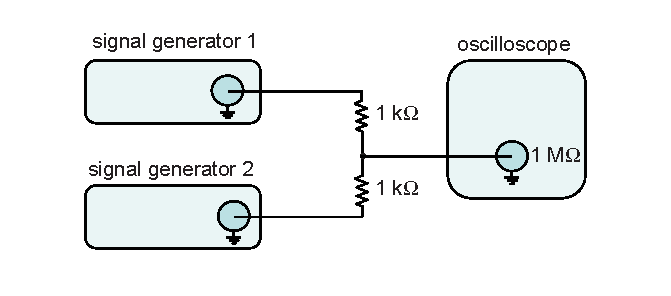
\includegraphics[width=4in]{sumcircuitfig.eps}
\caption{\label{sumcircuit} 
Example diagram of a circuit that combines the outputs of two
function generators to achieve a sum of the two waveforms.}
\end{figure}

Connect two function generators to produce a combined signal as input to
the data acquisition board.  You will need to use series resistors in order
to successfully combine the outputs, otherwise the two outputs will fight
each other.  The circuit shown in Fig.~\ref{sumcircuit} provides an example
of how this is done.  Set both function generators to give a sine wave output
of approximately equal amplitude of 0.5~V and a frequency of 3~kHz.
Describe qualitatively the output as seen on the oscilloscope. Have you seen
anything like this before? Change one frequency and observe the effect. Watch
the FFT output at the same time and describe what happens.

One great advantage of FFT spectral analysis is its ability to isolate a
small signal from a large background. Try this by setting one function
generator to an amplitude of 1~V and a frequency of 10~kHz (this will be
the background), and the other to as small an amplitude as the generator
will provide and a frequency of about 5~kHz (this will be the signal). On
the oscilloscope, the second signal will be barely visible as a tiny
modulation on top of the dominant 10~kHz sine wave. Now look at the Fourier
spectrum and record what you see. Estimate how small a 5~kHz signal can be
detected using the FFT to isolate it.

\begin{acknowledgments}
This document was updated by Prof. Richard Jones, based on an original
write-up by Prof. Ed Eyler (2001), with updates by Prof. Doug Hamilton (2005).
Prof. Ed Eyler acknowledges that the idea for this experiment originated from
a laboratory exercise for Physics 326 at Bucknell University. The work of
Professor E. Eyler in writing the data acquisition program is cheerfully
acknowledged.
\end{acknowledgments}

%% Create the reference section using BibTeX:
%\bibliography{revtex4}

\begin{thebibliography}{9}

\bibitem{Cooley65}
J.W.~Cooley and O.W.~Tukey, {\em An Algorithm for the Machine Calculation of
Complex Fourier Series}, Math.\ Comput.\ {\bf 19} (1965) pp.\ 297-301.
\bibitem{Thompson92}
W.J.~Thompson, {\em Fourier series and the Gibbs Phenomenon}, 
Am. J. Phys. {\bf 60} (1992) pp.\ 425-429.

\end{thebibliography}

\appendix

\section{Square Wave}

\begin{figure}
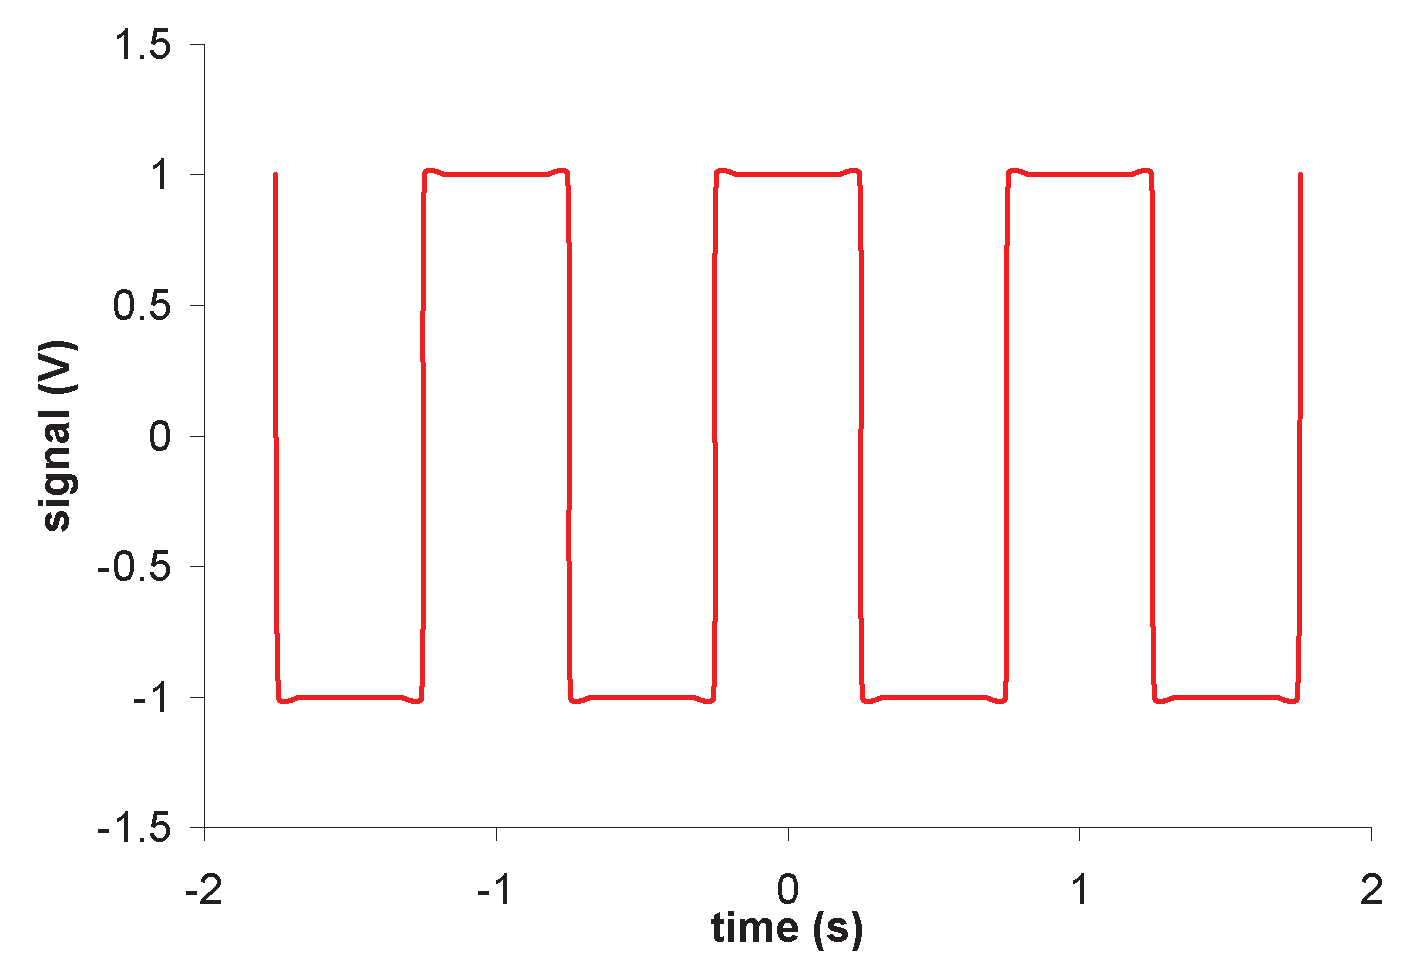
\includegraphics[width=6cm]{sqrwavefig.eps}
\caption{\label{sqrwavefig} 
Graph of a square wave of unit amplitude and period $T=1.0$~s.}
\end{figure}

The square wave illustrated in Fig.~\ref{sqrwavefig} has a duty cycle of
1.  The wave form is symmetric about $t=0$, so all of the $B_n$ coefficients
of the sine terms are zero.  By inspection of the figure, the time average
of the waveform is 0, so $A_0 = 0$. The Fourier series expansion of this
waveform, which has only odd harmonics, is
\begin{equation}
h(t) = -\frac{4}{\pi}\sum_{n=1,3,5,\ldots}^{\infty}
\frac{(-1)^{\frac{n+1}{2}}}{n}\cos\left(\frac{2\pi nt}{T}\right).
\label{eq:sqrwave}
\end{equation}

\section{Triangle Wave}

\begin{figure}
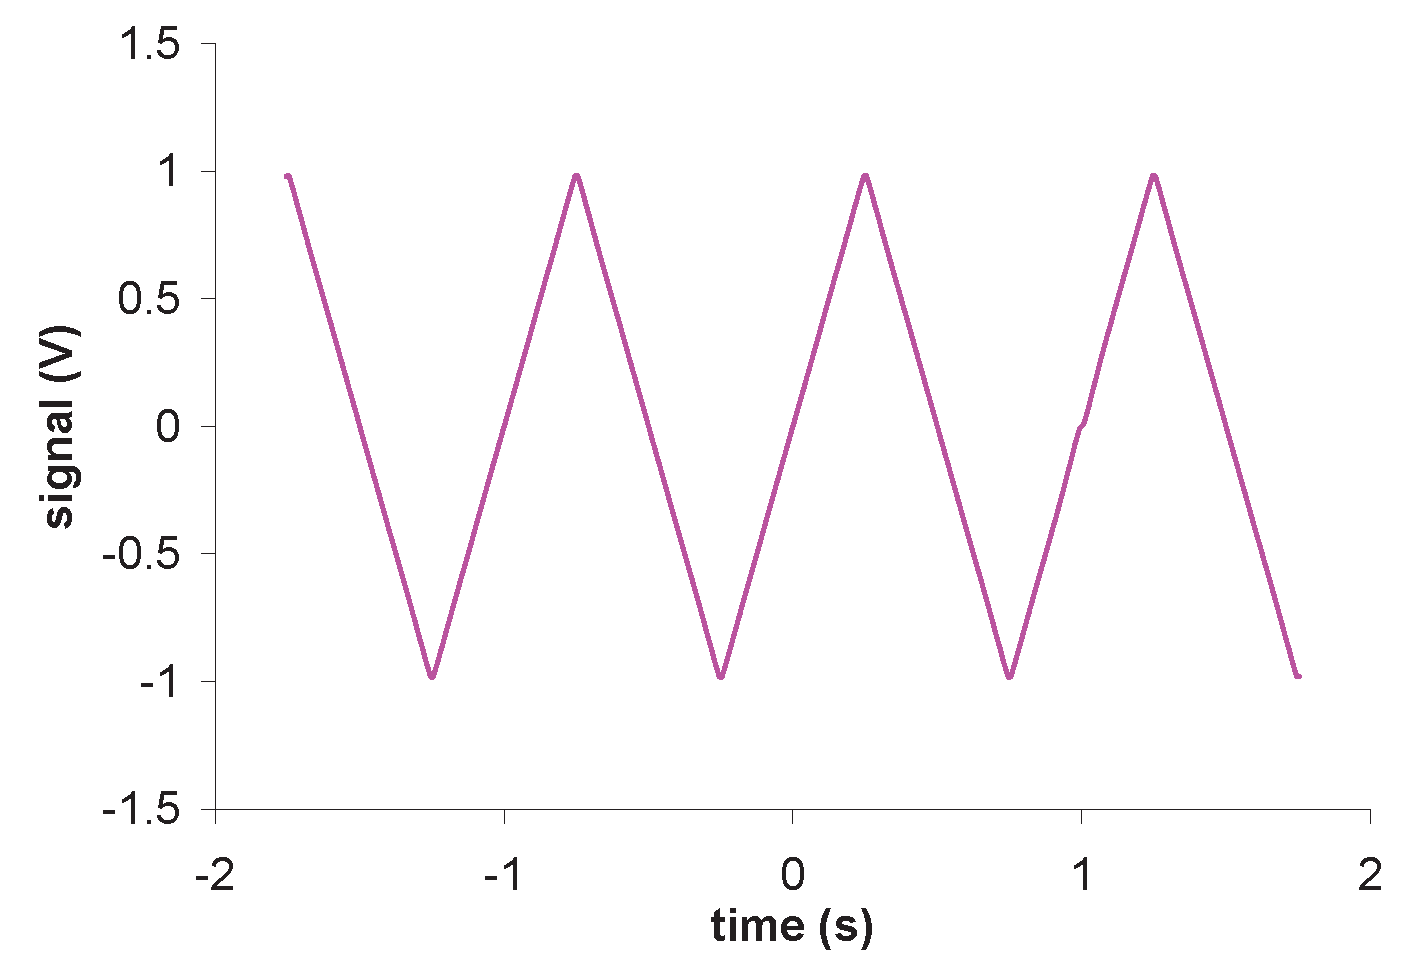
\includegraphics[width=6cm]{triwavefig.eps}
\caption{\label{triwavefig} 
Graph of a triangle wave of unit amplitude and period $T=1.0$~s.}
\end{figure}

The triangle wave illustrated in Fig.~\ref{triwavefig} has a duty cycle of
1. It is antisymmetric about t = 0 and thus contains only sine terms in its
Fourier expansion. Also note that the {\em dc} term $A_0$ is zero. 
The Fourier series for this waveform is
\begin{equation}
h(t) = \frac{8}{\pi^2}\sum_{n=1,3,5,\ldots}^{\infty}
\frac{(-1)^{\frac{n+1}{2}}}{n^2}\sin\left(\frac{2\pi nt}{T}\right)
\label{eq:triwave}
\end{equation}

\section{Sawtooth Wave}

\begin{figure}
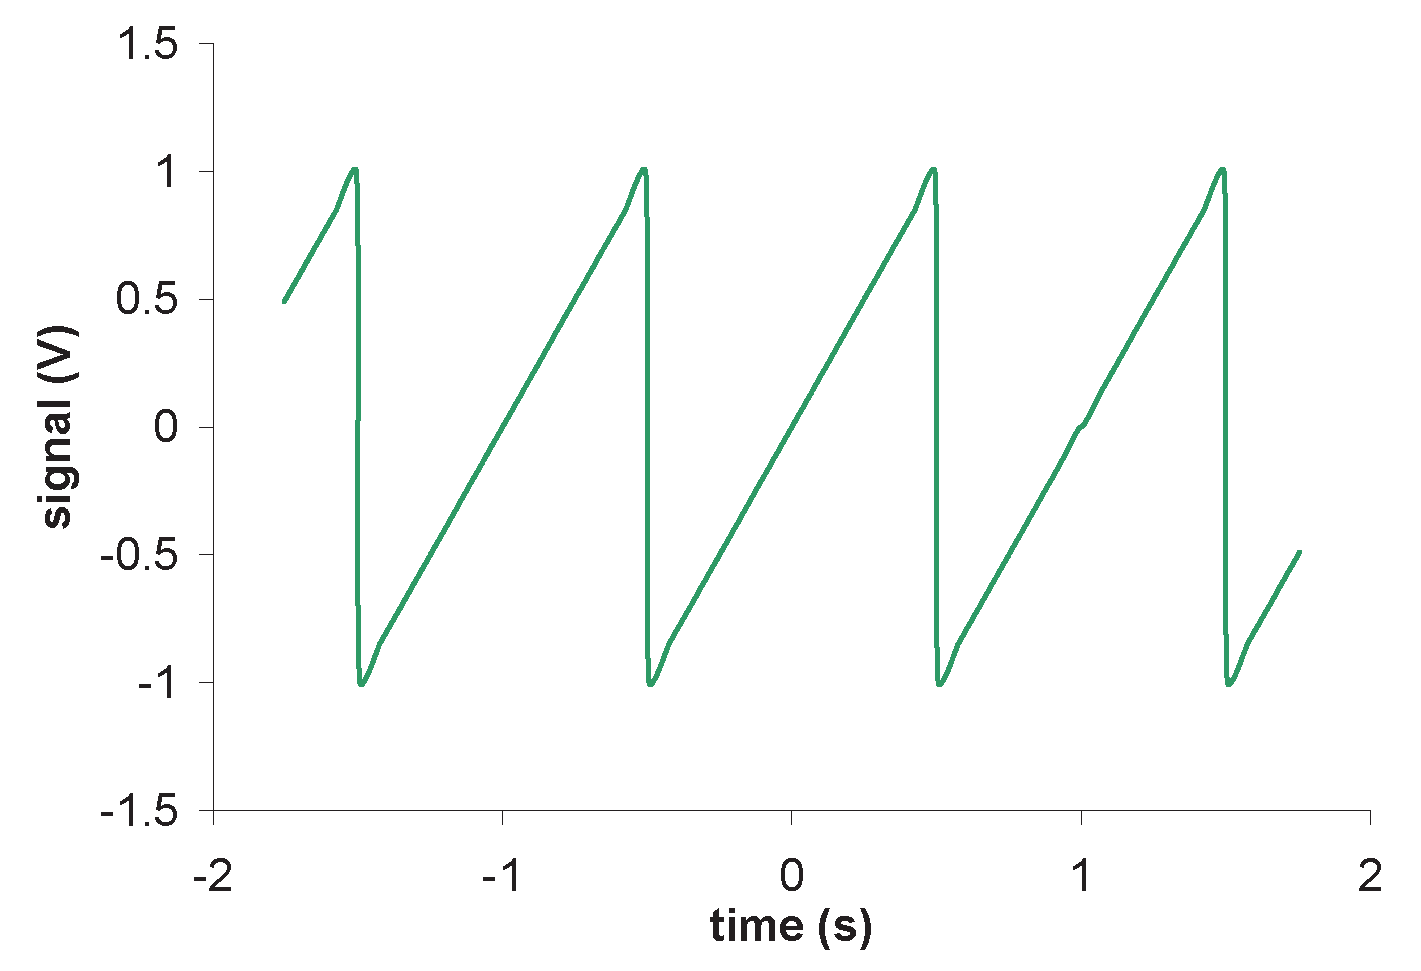
\includegraphics[width=6cm]{sawwavefig.eps}
\caption{\label{sawwavefig} 
Graph of a sawtooth wave of unit amplitude and period $T=1.0$~s.}
\end{figure}

The sawtooth wave defined in Eq.~\ref{eq:sawwave} is illustrated in
the Fig.~\ref{sawwavefig}.  It is clearly an antisymmetric function
whose time-average value is zero. The derivation of the Fourier series
is assigned to the student.

\section{Half-wave Rectified Sine Wave}

\begin{figure}
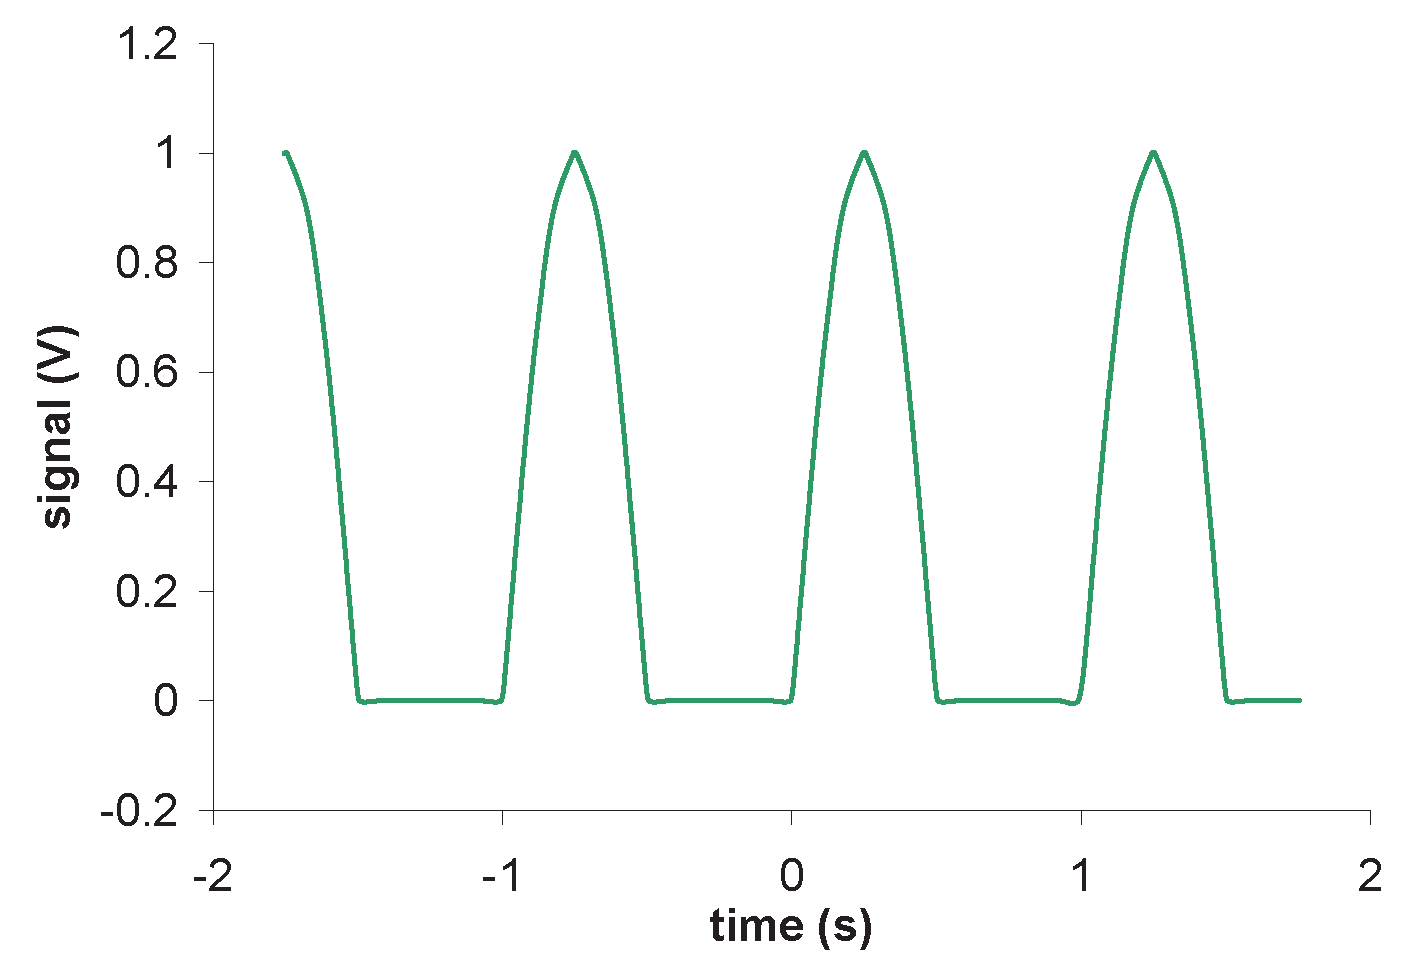
\includegraphics[width=6cm]{rsinwavefig.eps}
\caption{\label{rsinwavefig} 
Graph of a half-wave rectified sine wave of unit amplitude
and period $T=1.0$~s.}
\end{figure}

The half-wave rectified sine wave shown in Fig.~\ref{rsinwavefig}
is neither symmetric or antisymmetric.  Thus cosine and sine waves
must contribute in its Fourier series.  Also note that waveform has a
non-zero average value. The Fourier series representation is
\begin{equation}
h(t) = \frac{1}{\pi}+\frac{1}{2}\sin\left(\frac{2\pi t}{T}\right)
-\frac{2}{\pi}\sum_{n=2,4,\ldots}^{\infty}\frac{1}{n^2-1}
\cos\left(\frac{2\pi nt}{T}\right).
\label{eq:rsinwave}
\end{equation}

In comparison, a half-wave rectified cosine wave is symmetric about
$t = 0$ and thus contains only cosine terms in addition to the
{\em dc} term.

\end{document}
%%
%% ****** End of file template.aps ******
%
%
